% Agent–Environment interaction diagram – PPT colour scheme (v4 CUTE)
% Compile: xelatex agent_environment_tikz_v4.tex
% Convert: pdf2svg agent_environment_tikz_v4.pdf agent_environment_tikz_v4.svg
\documentclass[border=10pt]{standalone}
\usepackage{fontspec}
\setmainfont{Aptos}[
  Path = /Applications/Microsoft Word.app/Contents/Resources/DFonts/,
  Extension = .ttf,
  UprightFont = Aptos,
  BoldFont = Aptos-Bold,
  ItalicFont = Aptos-Italic,
  BoldItalicFont = Aptos-Bold-Italic,
]
\usepackage{amsmath,amssymb}
\usepackage{tikz}
\usetikzlibrary{arrows.meta, calc}

% PPT colours
\definecolor{accent}{HTML}{CB8044}
\definecolor{fg}{HTML}{E8E8E8}
\definecolor{fgdim}{HTML}{AAAAAA}
% Robot
\definecolor{robotbody}{HTML}{3A3A3A}
\definecolor{robotlight}{HTML}{505050}
\definecolor{cheek}{HTML}{E8956A}
% Globe
\definecolor{land}{HTML}{7BA656}
\definecolor{ocean}{HTML}{5C85A8}

\begin{document}
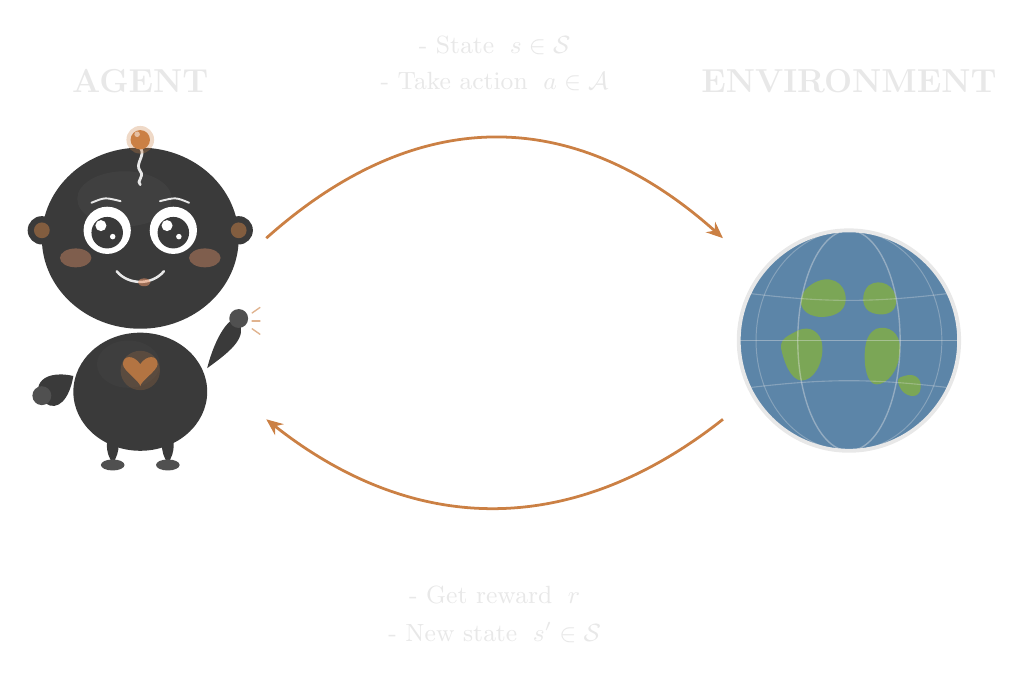
\begin{tikzpicture}[
    >=Stealth,
    curvedarrow/.style={
        accent,
        line width=1pt,
        -{Stealth[length=6pt, width=5pt]},
    },
]

% =============================================
% AGENT – THE CUTEST ROBOT
% =============================================
\begin{scope}[shift={(0,0.2)}, line cap=round, line join=round]

  % --- Big round head (chibi proportions: head > body) ---
  % Head fill – large, round, slightly wider than tall
  \fill[robotbody] (0,1.6) ellipse (1.25 and 1.15);
  % Slight highlight on forehead
  \fill[robotlight, opacity=0.3] (-0.2,2.1) ellipse (0.6 and 0.35);

  % --- Antenna: bouncy spring-like ---
  \draw[fg, line width=1pt] (0,2.75) .. controls (0.08,2.65) and (-0.08,2.55) .. (0,2.45)
    .. controls (0.06,2.38) and (-0.06,2.32) .. (0,2.28);
  % Antenna ball – glowing accent
  \fill[accent, opacity=0.3] (0,2.85) circle (5pt);
  \fill[accent] (0,2.85) circle (3.5pt);
  \fill[white, opacity=0.5] (-0.04,2.92) circle (1pt);

  % --- Ears: tiny round ones ---
  \fill[robotbody] (-1.25,1.7) circle (0.18);
  \fill[accent, opacity=0.5] (-1.25,1.7) circle (0.1);
  \fill[robotbody] (1.25,1.7) circle (0.18);
  \fill[accent, opacity=0.5] (1.25,1.7) circle (0.1);

  % --- Eyes: big round friendly eyes (symmetrical) ---
  % Left eye
  \fill[white] (-0.42,1.7) circle (0.3);
  \fill[robotbody] (-0.42,1.67) circle (0.2);
  \fill[white] (-0.5,1.76) circle (0.07);
  \fill[white] (-0.35,1.62) circle (0.035);
  % Right eye
  \fill[white] (0.42,1.7) circle (0.3);
  \fill[robotbody] (0.42,1.67) circle (0.2);
  \fill[white] (0.34,1.76) circle (0.07);
  \fill[white] (0.49,1.62) circle (0.035);

  % --- Tiny eyebrows (friendly, slightly raised) ---
  \draw[fg, line width=0.7pt] (-0.62,2.05) .. controls (-0.45,2.12) .. (-0.25,2.07);
  \draw[fg, line width=0.7pt] (0.62,2.05) .. controls (0.45,2.12) .. (0.25,2.07);

  % --- Rosy cheeks ---
  \fill[cheek, opacity=0.4] (-0.82,1.35) ellipse (0.2 and 0.12);
  \fill[cheek, opacity=0.4] (0.82,1.35) ellipse (0.2 and 0.12);

  % --- Mouth: sweet happy smile with open grin ---
  \fill[robotbody] (0,1.12) ellipse (0.22 and 0.12);
  \draw[fg, line width=0.9pt] (-0.3,1.18) .. controls (-0.15,1.0) and (0.15,1.0) .. (0.3,1.18);
  % Tongue
  \fill[cheek, opacity=0.55] (0.05,1.04) ellipse (0.08 and 0.05);

  % --- Body: small, round, bean-shaped (chibi = tiny body) ---
  \fill[robotbody] (0,-0.35) ellipse (0.85 and 0.75);
  \fill[robotlight, opacity=0.2] (-0.15,0.0) ellipse (0.4 and 0.3);

  % Heart on chest
  \fill[accent, opacity=0.8]
    (0,0.0) .. controls (-0.08,0.12) and (-0.22,0.12) .. (-0.22,0.0)
    .. controls (-0.22,-0.08) and (0,-0.22) .. (0,-0.28)
    .. controls (0,-0.22) and (0.22,-0.08) .. (0.22,0.0)
    .. controls (0.22,0.12) and (0.08,0.12) .. (0,0.0);
  % Heart glow
  \fill[accent, opacity=0.2] (0,-0.08) circle (0.25);

  % --- Arms: stubby, slightly raised (waving!) ---
  % Left arm – resting
  \fill[robotbody] (-0.85,-0.15)
    .. controls (-1.3,-0.05) and (-1.4,-0.35) .. (-1.2,-0.5)
    .. controls (-1.05,-0.6) and (-0.9,-0.45) .. (-0.85,-0.15);
  % Left hand – round
  \fill[robotlight] (-1.25,-0.4) circle (0.12);

  % Right arm – waving up!
  \fill[robotbody] (0.85,-0.05)
    .. controls (1.2,0.2) and (1.35,0.35) .. (1.25,0.55)
    .. controls (1.15,0.65) and (0.95,0.35) .. (0.85,-0.05);
  % Right hand – round, waving
  \fill[robotlight] (1.25,0.58) circle (0.12);
  % Tiny wave lines
  \draw[accent, line width=0.5pt, opacity=0.6] (1.42,0.65) -- (1.52,0.72);
  \draw[accent, line width=0.5pt, opacity=0.6] (1.42,0.55) -- (1.52,0.55);
  \draw[accent, line width=0.5pt, opacity=0.6] (1.42,0.45) -- (1.52,0.38);

  % --- Legs: short stubby ---
  \fill[robotbody] (-0.35,-1.0)
    .. controls (-0.45,-0.85) and (-0.45,-1.15) .. (-0.35,-1.25)
    .. controls (-0.25,-1.15) and (-0.25,-0.85) .. (-0.35,-1.0);
  \fill[robotlight] (-0.35,-1.28) ellipse (0.15 and 0.07);
  \fill[robotbody] (0.35,-1.0)
    .. controls (0.45,-0.85) and (0.45,-1.15) .. (0.35,-1.25)
    .. controls (0.25,-1.15) and (0.25,-0.85) .. (0.35,-1.0);
  \fill[robotlight] (0.35,-1.28) ellipse (0.15 and 0.07);

\end{scope}

% Agent label
\node[fg, font=\fontsize{12}{14}\selectfont\bfseries] at (0,3.8) {AGENT};

% =============================================
% ENVIRONMENT – Schematic globe with colours (same as v3)
% =============================================
\begin{scope}[shift={(9,0.5)}]
  % Ocean fill
  \fill[ocean] (0,0) circle (1.4);

  % Land mass blobs
  \fill[land] (-0.55,0.65)
    .. controls (-0.35,0.85) and (-0.1,0.8) .. (-0.05,0.6)
    .. controls (0.0,0.4) and (-0.15,0.3) .. (-0.35,0.3)
    .. controls (-0.55,0.3) and (-0.7,0.45) .. (-0.55,0.65);
  \fill[land] (0.25,0.7)
    .. controls (0.4,0.8) and (0.6,0.7) .. (0.6,0.5)
    .. controls (0.6,0.35) and (0.45,0.3) .. (0.3,0.35)
    .. controls (0.15,0.4) and (0.15,0.6) .. (0.25,0.7);
  \fill[land] (0.35,0.15)
    .. controls (0.5,0.2) and (0.65,0.1) .. (0.65,-0.1)
    .. controls (0.65,-0.3) and (0.55,-0.5) .. (0.4,-0.55)
    .. controls (0.25,-0.6) and (0.2,-0.4) .. (0.2,-0.2)
    .. controls (0.2,0.0) and (0.25,0.1) .. (0.35,0.15);
  \fill[land] (-0.7,0.1)
    .. controls (-0.55,0.2) and (-0.4,0.15) .. (-0.35,0.0)
    .. controls (-0.3,-0.2) and (-0.4,-0.45) .. (-0.55,-0.5)
    .. controls (-0.7,-0.55) and (-0.8,-0.35) .. (-0.85,-0.15)
    .. controls (-0.9,0.0) and (-0.8,0.05) .. (-0.7,0.1);
  \fill[land] (0.7,-0.45)
    .. controls (0.85,-0.4) and (0.95,-0.5) .. (0.9,-0.65)
    .. controls (0.85,-0.75) and (0.7,-0.7) .. (0.65,-0.6)
    .. controls (0.6,-0.5) and (0.62,-0.47) .. (0.7,-0.45);

  % Schematic grid lines
  \draw[fg, line width=0.5pt, opacity=0.4] (0,-1.4) arc[start angle=-90, end angle=90, x radius=0.65, y radius=1.4];
  \draw[fg, line width=0.5pt, opacity=0.4] (0,1.4) arc[start angle=90, end angle=270, x radius=0.65, y radius=1.4];
  \draw[fg, line width=0.35pt, opacity=0.3] (0,-1.4) arc[start angle=-90, end angle=90, x radius=1.18, y radius=1.4];
  \draw[fg, line width=0.35pt, opacity=0.3] (0,1.4) arc[start angle=90, end angle=270, x radius=1.18, y radius=1.4];
  \draw[fg, line width=0.5pt, opacity=0.4] (-1.4,0) -- (1.4,0);
  \draw[fg, line width=0.4pt, opacity=0.3] (-1.28,0.6) .. controls (-0.3,0.48) and (0.3,0.48) .. (1.28,0.6);
  \draw[fg, line width=0.4pt, opacity=0.3] (-1.28,-0.6) .. controls (-0.3,-0.48) and (0.3,-0.48) .. (1.28,-0.6);

  % Globe outline
  \draw[fg, line width=1.4pt] (0,0) circle (1.4);
\end{scope}

% Environment label
\node[fg, font=\fontsize{12}{14}\selectfont\bfseries] at (9,3.8) {ENVIRONMENT};

% =============================================
% TOP ARROW: Agent -> Environment
% =============================================
\draw[curvedarrow]
    (1.6,1.8) .. controls (3.5,3.5) and (5.5,3.5) .. (7.4,1.8);

% Top labels
\node[fg, font=\fontsize{9}{11}\selectfont, anchor=south] at (4.5,4.0) {%
  - State\; $s \in \mathcal{S}$%
};
\node[fg, font=\fontsize{9}{11}\selectfont, anchor=south] at (4.5,3.55) {%
  - Take action\; $a \in \mathcal{A}$%
};

% =============================================
% BOTTOM ARROW: Environment -> Agent
% =============================================
\draw[curvedarrow]
    (7.4,-0.5) .. controls (5.5,-2.0) and (3.5,-2.0) .. (1.6,-0.5);

% Bottom labels
\node[fg, font=\fontsize{9}{11}\selectfont, anchor=north] at (4.5,-2.5) {%
  - Get reward\; $r$%
};
\node[fg, font=\fontsize{9}{11}\selectfont, anchor=north] at (4.5,-2.95) {%
  - New state\; $s' \in \mathcal{S}$%
};

\end{tikzpicture}
\end{document}
